% !TeX root = thesis.tex
%--------------------------------------------------------------------%
%
% Template TA LaTeX Teknik Informatika ITERA.
% Editor: Radhinka Bagaskara, Martin C.T. Manullang, iwawiwi
% Version 2022-0.1
%
% Berdasarkan "Templat LaTeX Tesis Informatika ITB" oleh Petra Barus & Peb Ruswono Aryan
% https://github.com/petrabarus/if-itb-latex
%--------------------------------------------------------------------%
%
% Berkas ini berisi struktur utama dokumen LaTeX yang akan dibuat.
%
%--------------------------------------------------------------------%

\documentclass[12pt, a4paper, onecolumn, oneside, final]{report}

%-------------------------------------------------------------------%
%
% Konfigurasi dokumen LaTeX untuk laporan tesis IF ITB
%
% @author Petra Novandi
%
%-------------------------------------------------------------------%
%
% Berkas asli berasal dari Steven Lolong
%
%-------------------------------------------------------------------%

% Ukuran kertas
\special{papersize=210mm,297mm}

% Setting margin
\usepackage[top=3cm,bottom=3cm,left=4cm,right=3cm]{geometry}

\usepackage{mathptmx}

% Judul bahasa Indonesia
\usepackage[bahasa]{babel}

% Format citation
\usepackage[backend=bibtex,citestyle=ieee]{biblatex}

\usepackage[utf8]{inputenc}
\usepackage{graphicx}
\usepackage{titling}
\usepackage{blindtext}
\usepackage{sectsty}
\usepackage{chngcntr}
\usepackage{etoolbox}
\usepackage[bookmarks]{hyperref}
\hypersetup{
    colorlinks,
    citecolor=black,
    filecolor=black,
    linkcolor=black,
    urlcolor=black
}% Package untuk link di daftar isi.
\usepackage{titlesec}       % Package Format judul
\usepackage{parskip}
\usepackage{ragged2e}		% Alignment
\usepackage{multirow}		% Untuk bisa merge cell di tabel
\usepackage{tikz}			% Untuk menggambar kotak pas foto
\usepackage{setspace}
\newcommand{\dokumentspacing}{1.5}  % Nilai Spasi antar baris
\newcommand{\setdocumentspacing}{%
    \setstretch{\dokumentspacing}%
}
\usepackage{fancyhdr}		% Agar nomor halaman di pojok kanan atas
\usepackage{caption} 		% Caption gambar & tabel

% Setting supaya nomor halaman pertama dengan "chapter"
% berada di kanan atas
\fancypagestyle{plain}{%
	\fancyhf{}%
	\renewcommand{\headrulewidth}{0pt}
	\fancyhead[R]{\thepage}
}

% Line satu setengah spasi
\renewcommand{\baselinestretch}{1.5}

% Setting judul
\chapterfont{\centering \large}
\titleformat{\chapter}[display]%
  	{\large\centering\bfseries}%
  	{\chaptertitlename\ \thechapter}{0pt}%
  	{\large\bfseries\uppercase}
\titleformat{\section}%
	{\normalfont\normalsize\bfseries}{\thesection}{1em}{}
\titleformat{\subsection}%
	{\normalfont\normalsize\bfseries}{\thesubsection}{1em}{}
    
% Setting spacing di setiap judul chapter
\titlespacing*{\chapter}{0pt}{-30pt}{20pt}

% Setting nomor pada subbsubsubbab
\setcounter{secnumdepth}{3}

\makeatletter
% Command untuk variabel NIM
\newcommand{\nim}[1]{\def\@nim{#1}}
\newcommand{\printnim}{\@nim}

% Command untuk variabel Dosen Pembimbing I & II
\newcommand{\namadosbinga}[1]{\def\@namadosbinga{#1}}
\newcommand{\namadosbingb}[1]{\def\@namadosbingb{#1}}
\newcommand{\nipdosbinga}[1]{\def\@nipdosbinga{#1}}
\newcommand{\nipdosbingb}[1]{\def\@nipdosbingb{#1}}
\newcommand{\printnamadosbinga}{\@namadosbinga}
\newcommand{\printnamadosbingb}{\@namadosbingb}
\newcommand{\printnipdosbinga}{\@nipdosbinga}
\newcommand{\printnipdosbingb}{\@nipdosbingb}
\newcommand{\dosbingA}[2]{\namadosbinga{#1} \nipdosbinga{#2}}
\newcommand{\dosbingB}[2]{\namadosbingb{#1} \nipdosbingb{#2}}

\makeatother

% Counter untuk figure dan table.
\counterwithin{figure}{section}
\counterwithin{table}{section}

% Supaya tidak ada garis di header
\renewcommand{\headrulewidth}{0pt}

% Setting penomoran caption gambar
\renewcommand{\thefigure}{\arabic{chapter}.\arabic{figure}}

% Setting penomoran caption tabel
\renewcommand{\thetable}{\arabic{chapter}.\arabic{figure}}

% Mengkapitalkan judul Daftar Isi, Gambar, & Tabel
\addto\captionsbahasa{%
	\renewcommand{\contentsname}{DAFTAR ISI}%
	\renewcommand{\listfigurename}{DAFTAR GAMBAR}%
	\renewcommand{\listtablename}{DAFTAR TABEL}%
}

% english title
\providecommand\titleEN[1]{\providecommand\thetitleEN{#1}}

% Saya lupa ini buat apa (Radhinka)
%\renewcommand{\theHsection}{\thepart.section.\thesection}



\makeatletter

\makeatother

\bibliography{references}

\begin{document}
% 	\pagestyle{plain}
% 	\fancyhf{}
% 	\rfoot{Halaman \thepage}%

    %Basic configuration
    \title{Judul Tugas Akhir} 	% Judul Tugas Akhir
    \titleEN{Thesis Title}                  % Thesis Title
    \author{Nama Mahasiswa}		% Nama Mahasiswa
	\nim{1234567890}				% NIM Mahasiswa
	\dosbingA%
		{Nama dan Gelar Pembimbing I}%	% Nama Dosen Pembimbing 1
		{NIP. 123456789}				% NIP Dosen Pembimbing 1
	\dosbingB%
		{Nama dan Gelar Pembimbing II}%	% Nama Dosen Pembimbing 2
		{NIP. 123456789}				% NIP Dosen Pembimbing 2

    \pagenumbering{roman}
    \setcounter{page}{0}

    \clearpage
\pagestyle{empty}

\begin{center}
	\smallskip
	
	\begin{center}
		\fontsize{11pt}{11pt}
		\bfseries \MakeUppercase{\thetitle}
		\vfill
	    \uppercase{Tugas Akhir}
	    \vfill
		\normalfont Diajukan sebagai syarat menyelesaikan jenjang strata Satu (S-1) di Program Studi Teknik Informatika, Fakultas Teknologi Industri, Institut Teknologi Sumatera
		\vfill
	\end{center}

	\large \bfseries Oleh:\\
    \large \bfseries \theauthor\\
    \printnim
    \vfill
    
    \begin{figure}[h]
    	\centering
    	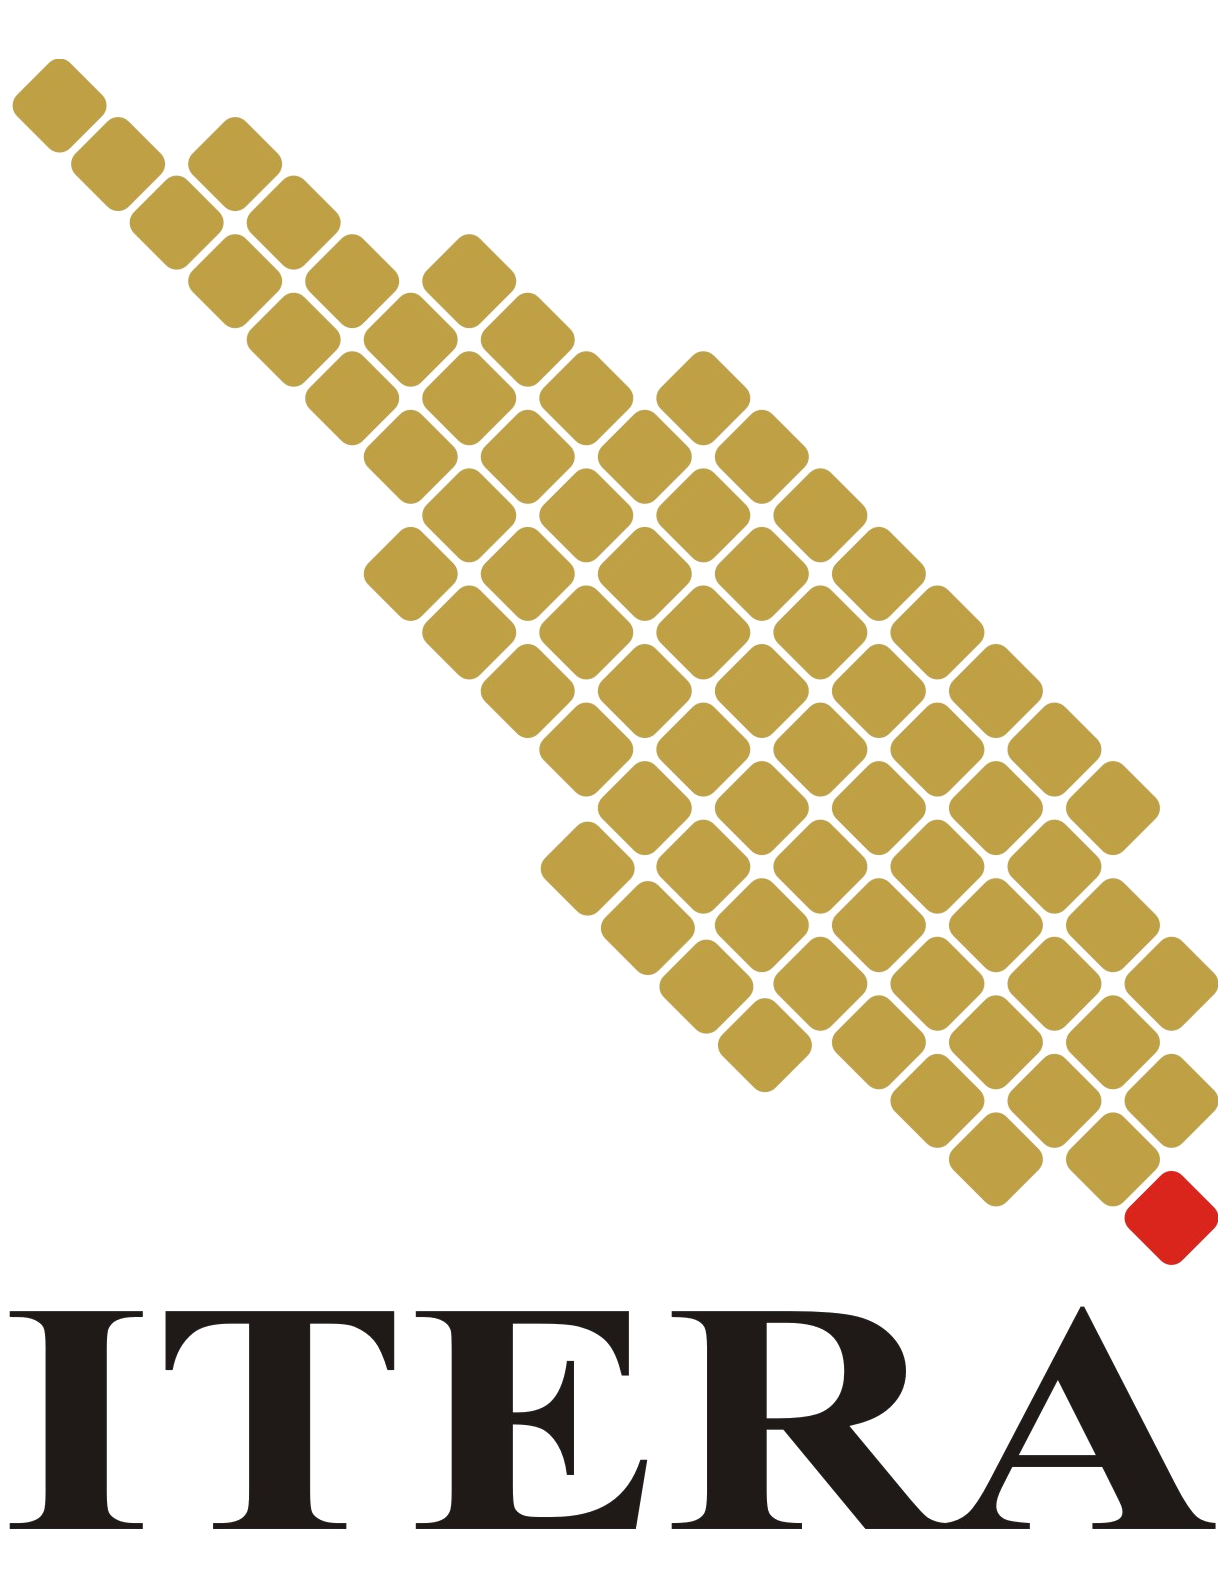
\includegraphics[width=3cm, keepaspectratio]{figure/Logo_ITERA.png}
    \end{figure}
    \vfill

	\begin{center}
		\fontsize{11pt}{11pt}
	    \bfseries
	    \uppercase{
	        Program Studi Teknik Informatika \\
	        Fakultas Teknologi Industri\\
	        Institut Teknologi Sumatera\\
	        Lampung Selatan
	    }\\
	    \the\year{}
    \end{center}

\end{center}

\clearpage
 % Hardcover
    \input{chapters/cover-soft} % Softcover
    \clearpage
\pagestyle{fancy}
\fancyhf{}
\fancyhead[R]{\thepage}
\phantomsection% 
\addcontentsline{toc}{chapter}{LEMBAR PENGESAHAN}

\begin{center}

	\large \bfseries \MakeUppercase{Lembar Pengesahan}
    
    \small \normalfont \singlespacing \justify{
    Saya menyatakan bahwa Tugas Akhir berjudul “{\thetitle}" merupakan hasil karya saya sendiri dan belum pernah diajukan, baik sebagian maupun seluruhnya, di Institut Teknologi Sumatera atau institusi pendidikan lain oleh saya maupun pihak lain.}
    %Tugas Akhir Sarjana dengan judul "{\thetitle}" adalah benar dibuat oleh saya sendiri dan belum pernah dibuat dan diserahkan sebelumnya, baik sebagian ataupun seluruhnya, baik oleh saya ataupun orang lain, baik di Institut Teknologi Sumatera maupun di institusi pendidikan lainnya.

	% Informasi Mahasiswa
    \flushleft
	\setlength{\tabcolsep}{0pt}
	\begin{tabular}{p{0.59\textwidth} p{0.3\textwidth}}
        \vspace{0.1cm}
		Lampung Selatan, \today & %
		\multirow{6}{*}{
			% Kotak pasfoto 3x4
			\phantom{----------------------} % Amazing hack biar kotaknya ke kanan (RDB)
			\begin{tikzpicture}
				\draw rectangle (2cm,3cm) node[pos=0.5] {Foto 2x3};
			\end{tikzpicture}
		}\\
		Penulis, \\
		& \\
		& \\
		%& \\
		\theauthor\\
		NIM. \printnim
	\end{tabular}
	% Informasi Dosen
	\vspace{0.4cm}
        \begin{center}
        Diperiksa dan disetujui oleh,
        \end{center}
        \vspace{0.1cm}

	\justify
    \setlength{\tabcolsep}{0pt}
    \begin{tabular}{ m{0.5cm}  m{0.7\textwidth} >{\centering\arraybackslash}m{0.3\textwidth}}
        \multicolumn{2}{c}{\hspace*{70pt}Pembimbing} & \multicolumn{1}{c}{} \\[2pt]
		1. & \printnamadosbinga & \\
		 & \printnipdosbinga & ............... \\%[4pt]
		 & \\
		2. & \printnamadosbinga & \\
		& \printnipdosbinga & ............... \\%[4pt]
		& \\
		\multicolumn{2}{c}{\hspace*{70pt}Penguji} & \multicolumn{1}{c}{} \\[2pt]
		1. & \printnamapengujia & \\
		& \printnippengujia & ............... \\[4pt]
            %& \\
		2. & \printnamapengujib & \\
		& \printnippengujib & ............... \\
    \end{tabular}
%	\vfill

	\begin{center}
		\fontsize{10pt}{10pt}
        \vspace{0.45cm}
		Disahkan oleh,\\
		Koordinator Program Studi Teknik Informatika\\
		Fakultas Teknologi Industri\\
		Institut Teknologi Sumatera
		\vspace{1.8cm}\\
		Andika Setiawan, S.Kom., M.Cs. \\ % TODO: make automatic
		NIP. 19911127 2022 03 1 007 \\
	\end{center}
	\vfill

\end{center}
\clearpage
    \input{chapters/statement}
    \input{chapters/publication}

    \clearpage
\phantomsection% 
\addcontentsline{toc}{chapter}{ABSTRAK}
\thispagestyle{fancy}

\begin{center}
	\large \bfseries \MakeUppercase{Abstrak}\\
	\normalsize \normalfont {\thetitle}\\
	\normalsize \normalfont {\theauthor}\\
	\bigskip
	
	\normalsize \normalfont \justifying \singlespacing
	Halaman ABSTRAK berisi uraian tentang latar belakang, tujuan, metodologi penelitian, hasil / kesimpulan. Ditulis dalam BAHASA INDONESIA tidak lebih dari 250 kata, dengan jarak antar baris satu spasi. Pada akhir abstrak ditulis kata “Kata Kunci” yang dicetak tebal, diikuti tanda titik dua dan kata kunci yang tidak lebih dari 5 kata. Kata kunci terdiri dari kata-kata yang khusus menunjukkan dan berkaitan dengan bahan yang diteliti, metode/instrumen yang digunakan, topik penelitian. Kata kunci diketik pada jarak dua spasi dari baris akhir isi abstrak.\par

    \vspace{20pt}
	\raggedright \textbf{Kata Kunci: kunci1, kunci2}
	
	\vfill
	
\end{center}
\clearpage
    \clearpage
\phantomsection% 
\addcontentsline{toc}{chapter}{ABSTRACT}
\thispagestyle{fancy}

\begin{center}
	\large \bfseries \MakeUppercase{Abstract}\\
	\normalsize \normalfont {\thetitleEN}\\
	\normalsize \normalfont {\theauthor}\\
	\bigskip
	
	\normalsize \normalfont \justifying \singlespacing
	Halaman ABSTRACT berisi uraian tentang latar belakang, tujuan, metodologi penelitian, hasil / kesimpulan. Ditulis dalam BAHASA INGGRIS tidak lebih dari 250 kata, dengan jarak antar baris satu spasi. Secara khusus, kata dan kalimat pada halaman ini tidak perlu ditulis dengan huruf miring meskipun menggunakan Bahasa Inggris, kecuali terdapat huruf asing lain yang ditulis dengan huruf miring (misalnya huruf Latin atau Greek, dll). Pada akhir abstract ditulis kata “Keywords” yang dicetak tebal, diikuti tanda titik dua dan kata kunci yang tidak lebih dari 5 kata. Keywords terdiri dari kata-kata yang khusus menunjukkan dan berkaitan dengan bahan yang diteliti, metode/instrumen yang digunakan, topik penelitian. Keywords diketik pada jarak dua spasi dari baris akhir isi abstrak.\par
    
    \vspace{20pt}
	\raggedright\textbf{Keywords: keywords1, keywords2}
	
	\vfill
	
\end{center}
\clearpage
    \input{chapters/motto}
    \input{chapters/dedicated}
    \clearpage
\phantomsection% 
\addcontentsline{toc}{chapter}{KATA PENGANTAR}
%\thispagestyle{fancy}

\begin{justifying}
	\large \bfseries \centering \MakeUppercase{Kata Pengantar}\linebreak
	
	\normalsize \normalfont \justifying
	\textit{Pada halaman ini mahasiswa berkesempatan untuk menyatakan terima kasih secara tertulis kepada pembimbing dan pihak lain yang telah memberi bimbingan, nasihat, saran dan kritik, kepada mereka yang telah membantu melakukan penelitian, kepada perorangan atau lembaga yang telah memberi bantuan keuangan, materi dan/atau sarana. Cara menulis kata pengantar beraneka ragam, tetapi hendaknya menggunakan kalimat yang baku. Ucapan terima kasih agar dibuat tidak berlebihan dan dibatasi pada pihak yang terkait secara ilmiah (berhubungan dengan subjek/materi penelitian). } \par
	Puji syukur kehadirat Allah SWT/Tuhan Yang Maha Esa atas limpahan rahmat, karunia, serta petunjuk-Nya sehingga penyusunan tugas akhir ini telah terselesaikan dengan baik. Dalam penyusunan tugas akhir ini penulis telah banyak mendapatkan arahan, bantuan, serta dukungan dari berbagai pihak. Oleh karena itu pada kesempatan ini penulis mengucapan terima kasih kepada: \par
	\begin{enumerate}
		\item {[Rektor ITERA]} selaku Rektor Institut Teknologi Sumatera.  
		\item {[Dekan FTI]} selaku Dekan Fakultas Teknologi Industri.
		\item {[Koor Prodi IF]} selaku Ketua Program Studi Teknik Informatika.
		\item {[Dosen Pembimbing]} selaku Dosen Pembimbing atas ide, waktu, tenaga, perhatian, dan masukan yang telah disumbangsihkan kepada penulis.
		\item {[Isi nama lainnya]}
	\end{enumerate} \par
	Akhir kata penulis berharap semoga tugas akhir ini dapat memberikan manfaat bagi kita semua.
	\vfill
	
\end{justifying}
\clearpage





\begin{comment}
\clearpage
\pagestyle{fancy}
\fancyhf{}
\fancyhead[R]{\thepage}
\phantomsection% 
%\clearpage
%\phantomsection% 
\addcontentsline{toc}{chapter}{KATA PENGANTAR}
%\thispagestyle{fancy}

\begin{justifying}
	\large \bfseries \centering \MakeUppercase{Kata Pengantar}\linebreak
	
	\normalsize \normalfont \justifying
	Puji syukur kehadirat Tuhan Yang Maha Esa atas limpahan rahmat, karunia, serta petunjuk-Nya sehingga penyusunan tugas akhir ini telah terselesaikan dengan baik. Dalam penyusunan tugas akhir ini penulis telah banyak mendapatkan arahan, bantuan, serta dukungan dari berbagai pihak. Oleh karena itu pada kesempatan ini penulis mengucapan terima kasih kepada: \par
	\begin{enumerate}
		\item Bapak Prof. Dr. I. Nyoman Pugeg Aryantha selaku Rektor Institut Teknologi Sumatera.  
		\item Bapak Hadi Teguh Yudistira, S.T., Ph.D. selaku Dekan Fakultas Teknologi Industri.
		\item Bapak Andika Setiawan, S. Kom., M. Cs. selaku Ketua Program Studi Teknik Informatika.
		\item Bapak Ilham Firman Ashari, S. Kom., M.T. selaku Koordinator Tugas Akhir Program Studi Teknik Informatika.  
		\item Bapak Martin C. T. Manullang, Ph.D. selaku Dosen Pembimbing atas ide, waktu, tenaga, perhatian, dan masukan yang telah disumbangsihkan kepada penulis.
            \item Bapak Andika Setiawan, S. Kom., M. Cs dan Bapak Eko Dwi Nugroho, S.Kom., M.Cs. selaku Dosen Penguji atas saran dan masukan yang diberikan. 
		\item Kedua Orang Tua dan Adik yang selalu memberikan dukungan dan doa sehingga penulis dapat menyelesaikan tugas akhir ini. Kelembutan, dukungan, dan cinta yang kalian berikan selalu menjadi sumber inspirasi dan kekuatan.
		\item Teman-teman penulis yang membantu selama masa perkuliahan yang tidak bisa disebutkan satu persatu.
	\end{enumerate} \par
	Akhir kata penulis berharap semoga tugas akhir ini dapat memberikan manfaat bagi kita semua. Penulis menyadari bahwa tugas akhir ini tidak luput dari kekurangan dan kelemahan, dan penulis  terbuka untuk menerima saran, kritik, dan masukan yang membangun.
	\vfill
	
\end{justifying}
\clearpage
\end{comment}

    \tableofcontents
    \listoffigures
    \listoftables
    \input{chapters/symbols}

    %----------------------------------------------------------------%
    % Konfigurasi Bab
    %----------------------------------------------------------------%
    \renewcommand{\chaptername}{BAB}
    % Bab: Arabic
    \renewcommand{\thechapter}{\Roman{chapter}}
    % Sub-bab: Roman
    \renewcommand\thesection{\arabic{chapter}.\arabic{section}}
    
    % Setting supaya nomor halaman pertama dengan "chapter"
    % berada di tengah bawah
    \fancypagestyle{plain}{%
    	\fancyhf{}%
    	\renewcommand{\headrulewidth}{0pt}
    	\fancyhead[]{}
    	\fancyfoot[C]{\thepage}
    }
    %----------------------------------------------------------------%

    %----------------------------------------------------------------%
    % Daftar Bab
    % Untuk menambahkan daftar bab, buat berkas bab misalnya `chapter-6` di direktori `chapters`, dan masukkan ke sini.
    %----------------------------------------------------------------%
    \setdocumentspacing
    \justifying
    \newpage
\pagestyle{fancy}
\fancyhf{}
\fancyhead[R]{\thepage}
\chapter{PENDAHULUAN} \label{Bab I}

\section{Latar Belakang} \label{I.Latar Belakang}
\textit{Mean Absolute Error} (MAE) \cite{knuth2001art}
\lipsum[1-3] % Menampilkan paragraf 1 sampai 2 dari lorem ipsum


\section{Rumusan Masalah} \label{I.Rumusan Masalah}

Berdasarkan latar belakang yang telah diuraikan di atas, maka permasalahan penelitian dirumuskan sebagai berikut: \par

\begin{enumerate}[noitemsep]
	\item Bagaimana
	\item Bagaimana 
\end{enumerate}


\section{Tujuan Penelitian} \label{I.Tujuan}
Berdasarkan rumusan masalah yang telah diuraikan di atas, maka tujuan dari penelitian ini adalah: \par

\begin{enumerate}[noitemsep]
	\item Menentukan 
	\item Mengimplementasikan
\end{enumerate}


\section{Batasan Masalah} \label{I.Batasan}
Adapun batasan masalah dari penelitian ini agar sesuai dengan yang diharapkan adalah sebagai berikut: \par

\begin{enumerate}[noitemsep]
    \item Bahasa pemrograman yang digunakan adalah bahasa pemrograman Python.
    \item 
\end{enumerate}


\section{Manfaat Penelitian} \label{I.Manfaat}
Adapun manfaat yang diperoleh dari hasil penelitian ini adalah sebagai berikut: \par

\begin{enumerate}[noitemsep]
    \item Menghasilkan sistem 
    \item 
\end{enumerate}


\section{Sistematika Penulisan} \label{I.Sistematika}
Sistematika penulisan berisi pembahasan apa yang akan ditulis disetiap Bab. Sistematika pada umumnya berupa paragraf yang setiap paragraf mencerminkan bahasan setiap Bab. \par

\noindent\textbf{Bab I}

Bab ini berisikan penjelasan latar belakang dari topik penelitian yang berlangsung, rumusan masalah dari masalah yang dihadapi pada penjelasan di latar belakang, tujuan dari penelitian, batasan dari penelitian, manfaat dari hasil penelitian, dan sistematika penulisan tugas akhir. \par

\noindent\textbf{Bab II}

Bab ini membahas mengenai teori-teori dan penelitian yang berkaitan dengan penelitian ini.

\noindent\textbf{Bab III}

Bab ini berisikan penjelasan alur kerja sistem, alat dan data yang digunakan, metode yang digunakan, dan rancangan pengujian.

\noindent\textbf{Bab IV}

Bab ini membahas hasil implementasi dan pengujian dari penelitian yang dilakukan.

\noindent\textbf{Bab V}

Bab ini membahas kesimpulan dari hasil penelitian dan juga saran untuk penelitian selanjutnya.
    \newpage
\chapter{TINJAUAN PUSTAKA} \label{Bab II}

\section{Tinjauan Pustaka} \label{II.Tinjauan}
Berisi penelitian terdahulu yang menjadi konsep / pendukung penelitian yang dilakukan. Lakukan pembahasan secara sistematis dengan menjelaskan masalah apa yang diangkat di penelitian terdahulu, metode yang digunakan, kontribusi yang diberikan, serta analisis penulis terkait dengan keunggulan atau keterbatasannya. Tuangkan perbandingan penelitian terdahulu dengan penelitian yang akan dikerjakan, minimal 5 jurnal pembanding (4-5 tahun terakhir). Kemudian penulis sebaiknya melakukan rangkuman terutama terkait dengan peluang pengembangan atau tugas akhir yang akan dilakukan \par

Perujukan literatur dapat dilakukan dengan menambahkan entri baru dalam file \verb|references.bib|. Cara merujuk sitasi menggunakan \verb|\cite{nama label sitasi}|. Hasil sitasi seperti ini: \cite{knuth2001art}, \cite{Vogels2006Am}, atau \cite{Suryanto2019MAE}\cite{Ivanny2014Banding}. Daftar Pustaka hanya akan memunculkan sitasi yang direferensikan menggunakan command \verb|\cite{}|. \par

Tuliskan \textbf{judul jurnal, penulis jurnal, tahun jurnal terbit, penjelasan isi jurnal, metode penelitian, hasil penelitian \& pengujian}. \par
\begin{enumerate}[noitemsep]
	\item Sistem Informasi Pendaftaran Haji dan Umroh Di PT Multazam Sriwijaya Barakah Palembang Menggunakan Metode Rapid Application Development. \blindtext
	\item Sistem Informasi Umroh Di PT XYZ Lampung Menggunakan Metode Rapid Application Development. \blindtext
\end{enumerate}

Tabel ringkasan tinjauan pustaka ditulis setelah penjelasan masing-masing jurnal. \par
\begin{longtable}{| b{0.05\textwidth}|p{0.2\textwidth}|p{0.2\textwidth}|p{0.15\textwidth}|p{0.25\textwidth}|} % Longtable berguna agar tabel dapat terpotong di halaman baru
	\caption{Literasi Penelitian Terdahulu}
	\label{table:2.literasi}\\
	\hline
	\textbf{No.} & \textbf{Judul} & \textbf{Masalah} & \textbf{Metode} & \textbf{Hasil} \\
	\hline
	\endfirsthead % Header tabel untuk halaman pertama
	\hline
	\textbf{No.} & \textbf{Judul} & \textbf{Masalah} & \textbf{Metode} & \textbf{Hasil} \\
	\hline
	\endhead % Header tabel untuk halaman selanjutnya (repeat header row)
	1. & Sistem Informasi Pendaftaran Haji dan Umroh Di PT Multazam Sriwijaya Barakah Palembang Menggunakan Metode Rapid Application Development & Belum adanya sistem untuk pendaftaran haji \& umrah & Rapid Application Development & Sistem Informasi Pendaftaran Haji dan Umroh di PT Multazam Sriwijaya Barakah Palembang\\ 
	\hline
	2. & Sistem Informasi Umroh Di PT XYZ Lampung Menggunakan Metode Rapid Application Development & Belum adanya sistem untuk pendaftaran haji \& umrah & Rapid Application Development & Sistem Informasi Pendaftaran Umroh di PT XYZ Lampung\\ 
	\hline
	3. & Sistem Informasi Umroh Di PT XYZ Lampung Menggunakan Metode Rapid Application Development & Belum adanya sistem untuk pendaftaran haji \& umrah & Rapid Application Development & Sistem Informasi Pendaftaran Umroh di PT XYZ Lampung\\ 
	\hline
\end{longtable}

\section{Dasar Teori} \label{II.Teori}
Berisi teori/konsep yang berkaitan/digunakan dalam tugas akhir yang dikerjakan. Gunakanlah data melalui buku/jurnal referensi, publikasi tugas akhir, penelitian, buku, dan informasi web yang dapat dipertanggungjawabkan, hindari penggunaan dasar teori melalui tautan Wikipedia, surat kabar, atau portal berita, yang dapat memiliki isi yang tidak bersifat fakta. \par

\subsection{Teori 1} \label{II.Teori1}
Berikut adalah contoh penyisipan tabel menggunakan \verb|\begin{longtable}{}|: \par
	
	\begin{longtable}{|c|c|c|c|}
		\caption{Contoh Tabel}
		\label{table:2.contoh}\\
		\hline
		Col1 & Col2 & Col2 & Col3 \\
		\hline
		\endhead
		1 & 6 & 87837 & 787 \\ 
		\hline
		2 & 7 & 78 & 5415 \\
		\hline
		3 & 545 & 778 & 7507 \\
		\hline
		4 & 545 & 18744 & 7560 \\
		\hline
		5 & 88 & 788 & 6344 \\
		\hline
	\end{longtable}

\subsubsection{Subsubbab} \label{II.Teori1.1}
Berikut adalah contoh subsubbab. Ini adalah level subbab maksimal dalam laporan Tugas Akhir, dan tidak boleh lebih dalam. \par

Gambar \ref{fig:2.contoh} adalah contoh Gambar yang diambil dari internet yang harus dicantumkan sumbernya dan memiliki lisensi Creative Common. Jika gambar adalah milik peneliti lain atau tidak dibuat atau diambil sendiri maka peneliti wajib meminta izin kepada peneliti lain tersebut untuk mencantumkan gambar. Gunakan \verb|\begin{figure}| untuk memasukkan gambar. Gunakan \verb|\caption{[nama caption]}| untuk memberikan caption gambar. Nomor caption akan diurutkan secara otomatis. Jangan lupa untuk melabeli setiap gambar dengan \verb|\label{[nama label]}|, agar bisa direferensi menggunakan \verb|\ref{[nama label]}| \par
\begin{figure}[H] % Kalau menggunakan H, posisi gambar akan tepat dibawah teks
	\centering
	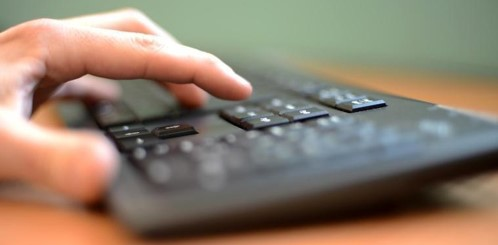
\includegraphics[width=0.6\textwidth]{figure/keyboard.jpg}
	\caption{Contoh gambar dan caption}
	\label{fig:2.contoh}
	{\footnotesize Sumber: Contoh} % Untuk memberikan sumber
\end{figure}

\subsection{Teori 2} \label{II.teori2}
Untuk membuat sebuah rumus persamaan, gunakan kode \verb|\begin{equationcaptioned}| seperti dibawah: \par
	
\begin{equationcaptioned}[eq:2.sederhana]{
	x + 1 = 2
}{
	Rumus sederhana % Caption rumus
}
\end{equationcaptioned}

Teks caption rumus tidak akan muncul di teks, tetapi akan muncul di Daftar Rumus. \par

\begin{equationcaptioned}[eq:2.mae]{
    MAE = \frac{1}{n} \sum_{i=1}^{n} \left| y_i - \hat{y}_i \right|
}{
    Mean Absolute Error (MAE)
}
\end{equationcaptioned}

Berikut adalah contoh penulisan persamaan yang lebih kompleks, yaitu persamaan distribusi normal. \par

\begin{equationcaptioned}[eq:2.mae]{
		P(x) = \frac{1}{{\sigma \sqrt {2\pi } }}e^{{{ - \left( {x - \mu } \right)^2 } \mathord{\left/ {\vphantom {{ - \left( {x - \mu } \right)^2 } {2\sigma ^2 }}} \right. \kern-\nulldelimiterspace} {2\sigma ^2 }}}
	}{
		Distribusi Normal
	}
\end{equationcaptioned}

Jika menuliskan banyak persamaan secara berurutan, gunakan  \verb|\begin{split}|: \par

\begin{equationcaptioned}[eq:2.mae]{
		\begin{split} 
			2x - 5y &=  8 \\ 
			3x + 9y &=  -12
		\end{split}
	}{
		Sistem persamaan linier
	}
\end{equationcaptioned}
    \newpage
\chapter{METODE PENELITIAN} \label{Bab III}

\section{Alur Penelitian} \label{III.Alur}
Pada penelitian ini, alur dirancang untuk memastikan setiap tahapan pemrosesan dilakukan secara sistematis dan efisien. Alur penelitian ini mencerminkan langkah-langkah utama terkait bagaimana proses yang dilakukan dalam penelitian, dari awal sampai dengan akhir. Gambarkan dalam bentuk diagram alir (\textit{flowchart}) seperti yang terlihat pada Gambar \ref{fig:3.alur}. \par

\begin{figure}[H] % Kalau menggunakan H, posisi gambar akan tepat dibawah teks
    \centering
    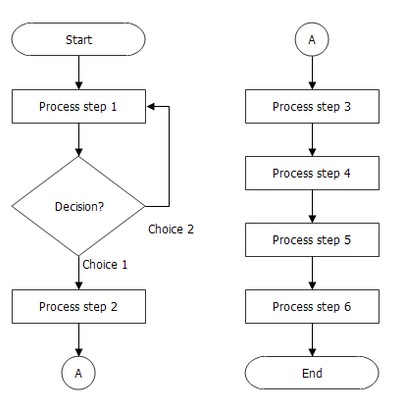
\includegraphics[width=0.6\textwidth]{figure/flowchart.jpg}
    \caption{Alur Penelitian}
    \label{fig:3.alur}
\end{figure}

\section{Penjabaran Langkah Penelitian} \label{III.Jabar Alur}
Jelaskan secara general langkah-langkah alur penelitian, yang sudah tergambar dalam flowchart di subbab \ref{III.Alur}. Subsubbab berikut harus sesuai dengan jumlah entitas langkah pada alur penelitian. \par

\subsection{Langkah 1} \label{III.Langkah 1}
Penjelasan Langkah 1. \par

\subsection{Langkah 2} \label{III.Langkah 2}
Penjelasan Langkah 2. \par

\section{Alat dan Bahan Tugas Akhir} \label{III.Alat dan Bahan}
Berisi alat-alat dan bahan-bahan yang digunakan dalam penelitian. \par

\subsection{Alat} \label{III.Alat}
Alat yang digunakan untuk melakukan penelitian, dapat berupa computer, PC, Arduino, raspberry, etc. Contoh: \par
\begin{enumerate}[noitemsep]
	\item \textit{Notebook} dengan spesifikasi minumum sistem operasi Windows 11, processor AMD Ryzen 5 7430 CPU @ 6 core/2,3 GHz, RAM 16GB DDR4, grafis AMD Radeon RX Vega 7 2GB, SSD 512 GB.
	\item \textit{Smartphone} dengan spesifikasi OS Android OS 12, CPU Snapdragon 778G Octa-core, GPU Adreno 642L, memori 128 GB, RAM 6 GB.
	\item Platform game engine Godot v4.3
	\item Code editor Microsoft Visual Studio Code
	\item Github
\end{enumerate}

\subsection{Bahan} \label{III.Bahan}
Bahan yang digunakan/diperlukan untuk melakukan penelitian, dapat berupa: \par
\begin{enumerate}[noitemsep]
	\item Dataset pihak lain yang diperoleh dengan izin atau dalam lisensi yang diizinkan untuk digunakan secara langsung,
	\item Dataset pihak pertama yang disusun sendiri melalui quisioner, observasi, atau interview,
	\item Dokumen panduan yang mengacu pada standar, hasil tugas akhir, atau artikel yang disitasi dan digunakan. 
\end{enumerate}

\section{Metode Pengembangan} \label{III.Metode}
Membahas mengenai metode yang digunakan dalam penelitian, berdasarkan dasar teori yang sebelumnya sudah dijelaskan pada subbab \ref{II.Teori}. Setiap Tugas Akhir wajib memiliki metode dalam pelaksanaannya yang sesuai dengan penelitian yang dikerjakan: \par
\begin{enumerate}[noitemsep]
	\item Alur pengembangan tugas akhir, menggunakan flowchart
	\item Cara pengumpulan data yang digunakan ()Kuesioner, Wawancara, pengujian, dan lainnya)
	\item Metode pengembangan tugas akhir (Metode Waterfall, Agile, RAD, dan lainnya).
\end{enumerate}
Subbab ini akan berhubungan erat dengan Subbab \ref{IV.Hasil}. \par

\section{Ilustrasi Perhitungan Metode} \label{III.Ilustrasi}
Dalam penelitian ini, hasil perhitungan dari program akan melalui serangkaian pengujian untuk mengevaluasi tingkat keakuratan model yang digunakan. Data dummy tersebut dapat dilihat pada Tabel \ref{table:3.dummy}. \par

\begin{longtable}{|c|c|c|c|c|c|c|c|c|}
	\caption{Data \textit{dummy} Pengujian}
	\label{table:3.dummy}\\
	\hline
	\multirow{2}{*}{\textbf{Subjek}} & \multicolumn{7}{|c|}{\textbf{Hasil Prediksi (BPM)}} & \multirow{2}{*}{\textbf{GT}} \\ \cline{2-8}
    & \textbf{F} & \textbf{NA} & \textbf{NO} & \textbf{RC} & \textbf{LC} & \textbf{M} & \textbf{C} & \\ 
        \hline
	   \endfirsthead
       \hline
       \multirow{2}{*}{\textbf{Subjek}} & \multicolumn{7}{|c|}{\textbf{Hasil Prediksi (BPM)}} & \multirow{2}{*}{\textbf{GT}} \\ \cline{2-8}
    & \textbf{F} & \textbf{NA} & \textbf{NO} & \textbf{RC} & \textbf{LC} & \textbf{M} & \textbf{C} & \\ 
    \hline
	\endhead
	\hline
	\endfoot
	\hline
	\endlastfoot
	1 & 68 & 69 & 68 & 70 & 68 & 71 & 69 & 68 \\ 
	\hline
	2 & 69 & 69 & 68 & 70 & 68 & 71 & 69 & 69 \\
	\hline
	3 & 70 & 70 & 69 & 71 & 68 & 73 & 69 & 70\\
	\hline
	4 & 71 & 70 & 70 & 72 & 69 & 73 & 70 & 71 \\
	\hline
	5 & 72 & 72 & 70 & 72 & 70 & 74 & 70 & 72 \\
	\hline
        6 & 73 & 72 & 71 & 74 & 71 & 76 & 71 & 73 \\ 
	\hline
	7 & 74 & 73 & 72 & 74 & 72 & 77 & 71 & 74 \\
	\hline
	8 & 75 & 74 & 72 & 74 & 73 & 77 & 73 & 75\\
	\hline
	9 & 76 & 75 & 73 & 75 & 74 & 78 & 75 & 76 \\
	\hline
	10 & 77 & 76 & 74 & 78 & 75 & 78 & 76 & 77
\end{longtable}
    \newpage
\chapter{HASIL DAN PEMBAHASAN} \label{Bab IV}

\section{Penggunaan Dataset} \label{IV.Penggunaan}
Dataset yang digunakan pada penelitian ini merupakan dataset PURE. 
\lipsum[1-2] % Menampilkan paragraf 1 sampai 2 dari lorem ipsum


\section{Akuisisi Gambar} \label{IV.Akuisisi}
Pada tahap ini, proses pembacaan dataset dilakukan dengan seksama untuk memastikan setiap gambar diperoleh dengan urutan yang benar dan sistematis. Penting untuk memastikan bahwa gambar yang diperoleh terurut dalam format \textit{time-series} agar memudahkan analisis pergerakan wajah yang terjadi dalam video. Implementasi kode yang digunakan untuk proses ini dapat dilihat pada \cref{code:4.contoh}. \par

% Menulis blok kode
\begin{lstlisting}[caption={Akuisisi Gambar}, label={code:4.contoh}]
def process_dataset(dataset_path):
	image_files = glob(os.path.join(dataset_path, '*.png'))
	image_files.sort()
	for image_file in image_files:
		frame = cv2.imread(image_file)
		if frame is None:
			continue
		frame_rgb = cv2.cvtColor(frame, cv2.COLOR_BGR2RGB)
		cv2.imshow('Frame', frame)
		if cv2.waitKey(1) & 0xFF == ord('q'):
			break
		cv2.destroyAllWindows()
def main():
    datasets = get_all_dataset_folders(DATASET_ROOT)
    for dataset in datasets:
        process_dataset(dataset)
        print("print string")
\end{lstlisting}


\section{Analisis Hasil Penelitian} \label{IV.Analisis}
\lipsum[1-2] % Menampilkan paragraf 1 sampai 2 dari lorem ipsum


\section{Pembahasan} \label{IV.Bahas}
\lipsum[1-2] % Menampilkan paragraf 1 sampai 2 dari lorem ipsum
    \newpage
\chapter{KESIMPULAN DAN SARAN} \label{Bab V}

\section{Kesimpulan} \label{V.Kesimpulan}
Berisi kesimpulan dari hasil dan pembahasan terkait penelitian yang dilakukan, dapat juga berupa temuan yang Anda dapatkan setelah melakukan penelitian atau analisis terhadap tugas akhir Anda. Memberikan jawaban dari poin pada subbab \nameref{I.Rumusan Masalah} dan \nameref{I.Tujuan}. \par

\section{Saran} \label{V.Saran}
Berisi saran mengenai aspek tugas akhir atau temuan yang dapat dikembangkan dan diperkaya di tugas akhir selanjutnya. Saran dapat berkaitan erat pada subbab \nameref{IV.Analisis}. \par
    %----------------------------------------------------------------%

    % Daftar pustaka
    \renewcommand{\bibname}{Daftar Pustaka}
    \phantomsection% 
    \addcontentsline{toc}{chapter}{Daftar Pustaka}
    \printbibliography

    % Index
    \appendix

    \addcontentsline{toc}{part}{Lampiran}
    \part*{Lampiran}

    \input{chapters/appendix-1}
    \input{chapters/appendix-2}

\end{document}
